\chapter{Literature Review}

\section{Content addressable Memory}
Content addressable memory also known as Associative memory , was first
proposed in the early 1960s by researchers at IBM, including Richard W. Harker,
Kenneth C. Thompson, and Robert D. Denny. Using the content of the data as the
address, CAM is a form of computer memory system that enables quick searching
and retrieval of data.

In traditional random access memory (RAM), data is stored in a specific
location based on a numerical address and the data can be retrieved by
accessing the corresponding address. In contrast, CAM stores data in a specific
location based on the content of the data and the data can be retrieved by
searching for the specific content rather than the numerical address.

CAM has several advantages over traditional RAM, including faster search and
retrieval times and the ability to store and retrieve data based on the content
rather than a numerical address. These features make CAM particularly useful in
applications where rapid searching and retrieval of data is important, such as
database management and pattern recognition.

The concept of CAM has had a significant impact on the field of computer
science. The work of Harker, Thompson and Denny has contributed to the
development of efficient and effective methods for storing and retrieving data
in computers. Its applications include database management systems which
require searching through the data as fast as possible
figure\ref{associative_circuit} shows one such circuit.
\begin{figure}[h!]
    \centering
    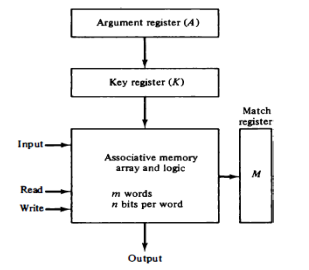
\includegraphics[width=0.7\linewidth]{associative}
    \caption{Associative memory circuit}\label{associative_circuit}
\end{figure}

\section{Associative network}
A particular kind of artificial neural network called an associative network is
made to store and retrieve data based on the strength of the connections
between neurons. Associative networks are frequently employed for tasks like
image recognition, natural language processing, and recommendation systems that
demand the recall of information based on the relationship and pattern.
\subsection{Influence of Context on Letter Perception:An Interactive Activation Model}
\subsubsection{Introduction}
The interactive activation model\cite{auto} is a computational model that
attempts to explain how the brain processes and interprets written language.
According to this theory, the brain stores and retrieves information about
letters and words based on the strength of the connections made between
neurons. The bottom-up and top-down processes have different impacts on the
strength of these connections.

The model proposes that the brain has a hierarchical structure, with
lower-level processing units representing features such as lines and curves,
and higher-level processing units representing letters and words. According to
the model, the activation of a processing unit depends on both the activation
of its inputs and the activation of its outputs.
\subsubsection{Proposed system}
The authors propose a hierarchical structure for the model, with lower-level
processing units representing features such as lines and curves, and
higher-level processing units representing letters and words. They contend that
a processing unit's activation is reliant on the activations of both its inputs
and outputs. The system's two primary ideas are

\begin{description}
    \item[Auto associative memory:]A single layer NN with the same number of training and
    output vectors. The weights are determined by the patterns to be stored.
    \item[Hetero associative memory:]A single-layer NN with different numbers of input
    training vectors and output vectors. The pattern stored in the network
    determines the weights. Because it is static, there will be no linear or delay
    operations.
\end{description}
\subsubsection{Advantages }
The model has the advantage of providing a computational framework for
understanding how the brain processes and interprets written language. It
suggests a hierarchical structure for the brain, with lower-level processing
units representing features such as lines and curves, and higher-level
processing units representing letters and words. Another advantage of the model
is that it is based on the concept of auto-associative and heteroassociative
memory, which are thought to be involved in how the human brain processes
language and perception. As a result, the model is able to capture the
intricate connections between letters and words and explain a variety of
occurrences in written language processing.

\subsubsection{Disadvantages}
A disadvantage of the model is that it is a simplified model of the brain, and
it may not capture all the complexity and nuance of language processing. It is
also based on a set of assumptions and simplifications, and it may not
accurately reflect the underlying mechanisms of the brain. In addition, the
model is based on a set of equations and learning rules that are used to
simulate the activation and deactivation of processing units, and these
equations may not mirror the brain's internal workings precisely.

\subsection{Neural networks and physical systems: The Hopfield network}
\subsubsection{Introduction}
The Hopfield model\cite{hopfield} is a type of RNN that is designed to mimic
the behaviour of neurons in the brain. It is a type of associative memory
system and hence it can store and recall information based on the relationship
between the data stored. It has applications including pattern recognition,
optimization, and error correction.
\subsubsection{Methodology}
The use of computational simulations and models to analyse the behaviour of
distributed systems, including neural networks, is covered in this article. He
suggested the Hopfield network, a sort of associative memory network. A
Hopfield network is made up of a collection of connected neurons arranged in a
single layer. Each neuron in the network is fully interconnected, and the
strength of the connections between neurons is dependent on the interactions
between inputs and outputs. A collection of equations that describe the
activation and deactivation of the neurons over time dictate the behaviour of a
Hopfield network. These equations are based on the idea of auto-associative
memory, where the original input can be retrieved from the output.
\subsubsection{Advantages}
The Hopfield model's relative simplicity and ease of implementation are two
benefits. It is made up of a single layer of fully linked neurons, and the
strength of the connections between them is determined by the interactions
between inputs and outputs. This simplicity makes the Hopfield model easy to
understand and implement. Another advantage of the Hopfield model is that it is
depending on the strength of the connections between neurons, is that it is
capable of storing and retrieving patterns or sequences of data. This makes it
useful for tasks that require the recall of specific patterns or sequences of
data, such as systems for recommendation, natural language processing, and
picture identification. Also, this model is relatively robust and resistant to
noise. These advantages make it useful in applications like image or speech
recognition systems.
\subsubsection{Disadvantages}
One disadvantage of the Hopfield model is that it is relatively simple and may
not be able to capture the complexity and nuance of more advanced neural
networks. Another drawback is that it can retrieve the information only with
the original input. A third disadvantage of the Hopfield model is that it can
be sensitive to initialization and may not always converge to a stable state
when used with a large amount or insufficiently distinct data. This can make it
difficult to use the model for certain types of tasks, such as optimization or
decision-making.
\section{Spiking neural network}
SNN are a subset of neural networks that mimic the behaviour of actual neurons
by encoding and transmitting information via spikes or pulses. They are a
relatively new variety of neural networks with the potential to raise the
effectiveness and performance of artificial intelligence systems. Building
associative memory systems using spiking neural networks is a relatively new
field of study that has only lately begun to attract attention.

\subsection{Training strategy for spiking neural networks for classification: SWAT }
\subsubsection{Introduction}
SWAT\cite{swat}(Spiking Weight association Training) is a method for training
spiking neural networks for classification tasks. To enhance SNN performance,
it combines supervised and unsupervised learning. Its foundation is the notion
that the network's input and output patterns can be used to modify the weights
of the connections between its neurons. The error between the network's actual
output and the desired output is taken into consideration when adjusting the
weights using a learning rule.
\subsubsection{Methodology}
They propose a method which merges Bienenstock-Cooper-Munro learning rule
(BCM)\cite{bcm} with Spike Time Dependent plasticity Spike-timing-dependent
plasticity (STDP)\cite{stdp}.The result is a weight distribution that is
unimodal, with weights and STDP being correlated.

The BCM learning rule is based on the notion that the network's connections
between neurons should be strengthened in accordance with the activity of those
neurons and the discrepancy between the network's actual output and the
anticipated output. The rule states that if the activity of the neurons is high
and the error is also high, the weights of the connections between neurons
should be increased, and if the activity of the neurons is low and the error is
also low, the weights should be decreased.

For neuromorphic computing, the research that is influenced by the structure
and operation of the brain, STDP is an unsupervised learning strategy based on
how neurons work in the brain. Based on the relative timing of spikes or
impulses, the strength of the connection between neurons fluctuates during the
process. The fundamental tenet of STDP is that if two $N_{prede}$ and
$N_{succe}$ neurons are connected, and their spike time are $w_1$ and $w_2$
respectively according to STDP \vspace*{-.3pc}
\begin{itemize}
    \item[]Strength of connection between $N_{prede}$ to $N_{succe}$ should  increase, if {\boldmath$w_1 w_2$}
    \item[]Strength of connection between $N_{prede}$ to $N_{succe}$ should  decrease, if {\boldmath$w_1<w_2$}
    \item[]Strength of connection between $N_{prede}$ to $N_{succe}$ should  remain same, if {\boldmath$w_1=w_2$}

\end{itemize}
%\vspace*{-2pc}

In general, the foundation of SWAT is the notion that the network's input and
output patterns can be used to modify the strength of connections between
neurons in the network. The error between the network's actual output and the
desired output is taken into consideration when adjusting the weights using
this rule.
\subsubsection{Advantages}
One of the main advantages of SWAT is that it spiking neural networks for
classification problems can be trained using this technique. Since SNN are a
promising sort of artificial neural network that is believed to have the
potential to enhance performance, therefore understanding this method is
crucial for better artificial intelligence systems. The network is trained
using a mix of supervised learning and unsupervised learning. As a result, the
network can both learn from tagged samples and independently find patterns and
features in the data.It is reasonably simple to execute and comprehend since it
is based on the straightforward learning rules of altering the weights of the
connections between neurons in the network based on the input and output
patterns of the network. Overall, it could make SNN use possible in a variety
of applications.
\subsubsection{Disadvantages}
Sometimes this may become computationally intensive, especially for large
networks with many neurons and connections. This could make it difficult to use
SWAT on systems with limited computational resources. Another potential
disadvantage is that it is based on supervised and unsupervised learning, when
efficient network training for supervised learning necessitates a significant
volume of labelled data. In some circumstances, getting this could be
challenging. It also depends on the network's initial weights for connections
between neurons, and the network's performance may be significantly impacted by
these weights. In order to obtain good performance, SWAT may be sensitive to
initialization and may need the initial weights to be carefully tuned.

\subsection{Backpropagation for spiking neural network:SpikeProp}
\subsubsection{Introduction}
Spiking neurons may be more biologically realistic and efficient than other
types of artificial neurons,additionally, they might be better suited for
specific jobs like pattern recognition and natural language processing.
However, they also note that training networks of spiking neurons can be
difficult due to the non-differentiable nature of the spiking function. To
address this problem, the authors propose the use of SpikeProp\cite{spikeprop},
which is a method for training networks of spiking neurons using
backpropagation.
\subsubsection{Methodology}
It is a technique for employing backpropagation to train networks of spiking
neurons. The spiking function, which describes the connection between a spiking
neuron's input and output, cannot be differentiated. This means that networks
of spiking neurons cannot be trained using conventional techniques for
artificial neural networks, such as backpropagation. But it can be used to
train networks of spiking neurons while avoiding this problem by using a
surrogate gradient function insted of the ordinary gradient ued in ANN. It
approximates the gradient of the spiking function.

\subsubsection{Advantages}
It enables the training of networks of spiking neurons using backpropagation.
This makes it possible to use backpropagation's ease of use and effectiveness
for training spiking neural networks. Spiking neural networks can be built
resembling more the biological systems than the conventional ANN and make it
better suited for particular tasks. It is also more efficient in training SNN
than other techniques. It makes it effective in applications like image
recognition and language translation.
\subsubsection{Disadvantages}
It is not effective in all applications of spiking neural networks. Also, due
to the approximations used in surrogate gradient function, it may not be always
accurate which may affect its performance.